%!TEX program = xelatex
%!TEX TS-program = xelatex
%!TEX encoding = UTF-8 Unicode

\documentclass[a4paper]{article}
\usepackage[UTF8, heading = false, scheme = plain]{ctex}
\usepackage{graphicx}
\usepackage{cite}
\usepackage{geometry}
\geometry{left=2.0cm, right=2.0cm, top=2.5cm, bottom=2.5cm}
\usepackage[colorlinks,linkcolor=red,anchorcolor=blue,citecolor=green]{hyperref}
\usepackage{subfig}
\usepackage{caption}
\captionsetup{font={scriptsize}}

\renewcommand\figurename{图}

\makeatletter
\let\@afterindentfalse\@afterindenttrue
\@afterindenttrue
\makeatother
\setlength{\parindent}{2em}  

\linespread{1.4}
\setlength{\parskip}{0.5\baselineskip}

\title{学习汇报\\第十五周}
\author{熊凯亚}
\date{\today}

\begin{document}
\maketitle
这周主要看了高级软件工程的作业要求看的论文\cite{ray2016naturalness}。

\section{摘要}
KLOC:千行代码,是一个程序有多大或者需要多少人来完成其编码工作的传统度量,可以用来衡量程序员生产效率。

一般为解决现实世界的问题二开发的应用程序,往往是自然的,高度重复的,并且是可预测的。研究人员通过统计模型捕获了软件的这种自然属性,并在建议引擎、移植工具、编码标准检查器和“习语”中使用它们。这表明,在某种意义上,对于一个好的统计语言模型来说,看似不可能的代码是“不自然的”,因此有可能是可疑的。本文对这一假设进行了研究。考虑来自10个不同Java项目的大量bug修复提交,并关注其语言统计,评估bug代码的自然特性和相应的Bug修复。本文研究发现,带有bug的代码往往熵值更大(即不自然),随着bug得到修复,它们变得更少。按平均熵对文件进行排序以获得成本效益评分,与流行的缺陷预测方法相当。在更细的粒度上,关注高度熵线与一些著名的静态bug查找程序(PMD、FindBugs)在成本效益上类似,使用熵度量对这些bug查找程序发出的警告进行排序可以提高检查包含在警告中的代码的成本效益。这表明熵可能是一种有效、简单的方法来补充PMD或FindBugs的有效性,并且基于搜索的bug修复方法可以从使用熵进行故障定位和查找修复中获益。

\section{引言}

代码仓库中的“自然”代码是高度重复的,这种重复可以被最初在统计自然语言处理(NLP)领域开发的语言模型有效地捕获。

当模型认为一个代码片段是不可能的时候,这意味着什么?

语言模型赋予代码更高的自然度(符号、语法形式等),在训练中经常遇到,而很少或从未见过的代码则更低的自然度。事实上,语法错误的代码被语言模型标记为不可能的。然而,通过限制自己的代码出现在存储库中,仍然会遇到不自然的,但语法上正确的代码;为什么?假设非自然代码更有可能是错误的,因此,语言模型实际上可以帮助消除潜在的缺陷代码。

这个概念似乎可信的;经验丰富的程序员在尝试诊断失败时,常常可以直观地忽略“看上去很滑稽”的代码。如果统计语言模型可以捕获这种能力,那么它们可以在各种设置中成为有用的辅助:它们可以改进缺陷预测;帮助为静态分析警告提供改进的优先级排序;改进故障定位算法的性能;甚至建议使用“更自然”的代码来替换有bug的代码。

为了研究这一现象,本文考虑了来自10个不同项目的7139个bugfix提交的大型文集,重点关注其语言统计,评估缺陷代码的自然性,以及修复是否增加了自然性。语言模型可以在任何粒度(甚至是字符级别)对语言事件的概率进行评级。本文关注行级的缺陷分析,与典型的统计缺陷预测方法相比,我们提供了更细的预测粒度,这些方法通常在文件或模块的粒度上操作。实际上,这种方法更适合静态分析或静态bug查找工具,它们也指示行级别上的潜在bug。出于这个原因,我们还对比研究了我们的语言模型方法,并结合了两个众所周知的静态bug查找器。

总的来说,结果证实了我们最初的假设,即带有bug的代码往往更不自然。

\section{背景}

行级别缺陷代码检测工具有:Static Bug Finer and Naturalness Bug Finder

本文研究的问题:中心问题是“不自然”(以熵或可改进性度量)是否表明代码质量较差?

Buggy Code:code that was implicated in bug fixes

\begin{enumerate}
\item Are buggy lines less “natural” than non-buggy lines? 含有Bug的代码行会比没有Bug的代码行更加不自然吗?

研究的结果会对基于搜索的自动化Bug修复产生影响:如果通过代码的自然性得知此代码更有可能修复,那么好的语言模型会为搜索提供有效的组织原则,甚至生成修复建议。
\item Are buggy lines less “natural" than bug-fix lines? Bug修复后的代码行会变得比以前更自然吗?

false positives (correct lines marked improbable);
false negatives (buggy lines indicated as natural)
\item Is “naturalness" a good way to direct inspection effort? 自然性是直接检验的好方法吗?

传统缺陷预测技术依赖于历史数据(如作者数量、更改历史、Bug),缺陷的预测是文件粒度的。我们可以以自然性作为原则,与行级别的SBF进行比较。
\item How do SBF and NBF compare in terms of ability to direct inspection effort? SBF和NBF从能力到预测检验的比较?

如果SBF在行级别发出警告,并且语言模型也认为不自然,我们可能会认为这行可能是错误的。

\item Is “naturalness" a useful way to focus the inspection effort on warnings produced by SBF? 对于SBF产生的警告,自然性是一种好的方式去专注于检验预测吗?

\end{enumerate}

\section{方法论}
\subsection{研究主题}
阶段一:考虑NBF的Bug查找能力
10个Java项目(5个来自Github,5个来自apache)活跃开发期一年的代码,每个月一个快照共120个。
考虑开发时和发行后NBF的Bug查找能力

阶段二:仅focus在发行后NBF作为Bug预测工具的性能

PMD operates on source code and produces line-level warnings; F IND B UGS operates on Java bytecode and reports warnings at line, method, and class level.

\subsection{数据收集}

阶段一:
\paragraph{估算Bug修复提交} 开发时Bug修复不会记录在Issue中,一般都是在commit中。因此,我们分析整个项目的每个commit并从中找出与Bug相关的关键字。首先将每个commit message转换成一个单词包,然后使用NLP对单词包进行分析。

\paragraph{识别快照中的错误行}
\begin{enumerate}
\item 识别与Bug相关的行(假设每次修复Bug都是行级别的)使用git diff,旧版标记为buggy,新版标记为fixed
\item 识别引入Bug的提交(使用 git-blame定位是哪些提交引入了这些Bug),如图\ref*{fig:data-collection}所示。
\item 将Bug行映射到相关快照
\end{enumerate}

\begin{figure*}[!h]
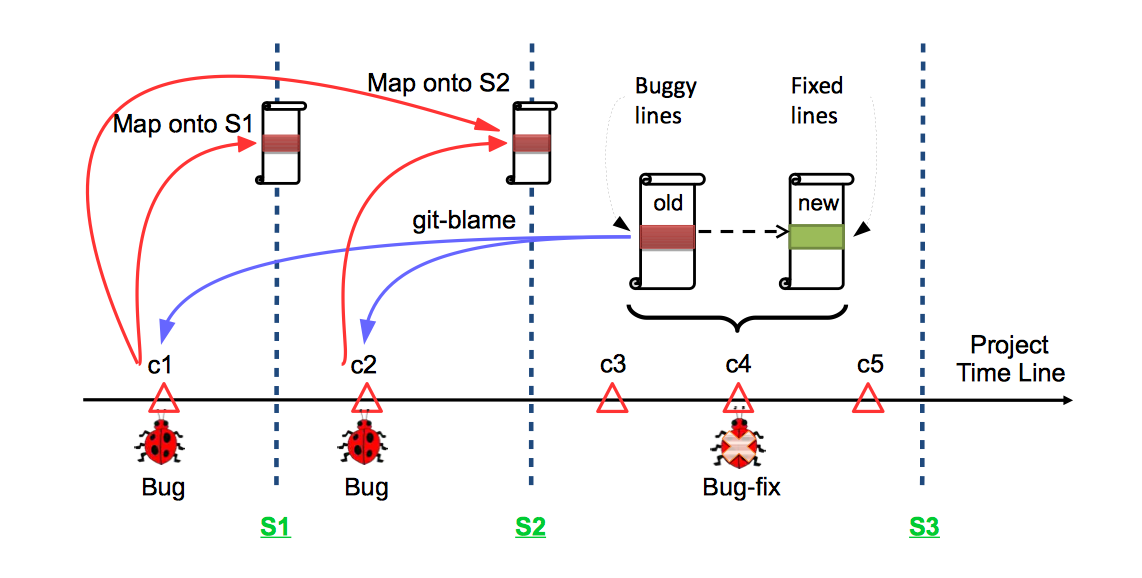
\includegraphics[width = \linewidth]{fig/data-collection.png}
\caption{收集Bug数据:纵向虚线是快照,三角形是每次提交。对于每一个修复Bug的提交,先使用git blame找出原先存在Bug的行(蓝色箭头),然后把他们映射到相应的快照上(红色箭头)}
\label{fig:data-collection}
\end{figure*}
注意:会遗漏一些出现并修复在snapshot interval中的Bug!!

阶段二:
对于阶段二,本文研究了Apache项目中发布后的bug。对于每一个发布,从JIRA的Issue追踪系统中找出修复Bug的提交,然后对于每一个发布版本找出Bug行和非Bug行。

\subsection{熵的度量}

使用\cite{tu2014localness}提出的基于缓冲的语言模型$\$gram$来度量熵。对于快照中给定的文件,这个工具首先基于快照中所有其他文件建立语言模型,然后通过在给定的文件上运行语言模型创建缓存(对本文件的习惯的缓存),并基于前一个token和后一个token计算每个token的熵。最后基于训练集和本地构建的缓存,这个工具计算出文件中每个token的熵,然后通过平均计算出每一行和每个文件的熵。

缓冲语言模型的影响因素包括:cache context, cache scope, cache size and cache order。 本文中是基于整个文件构建缓冲,因此只需要修改cache order参数即可。本文将缓冲的最大序列设置为10,最小补偿序列设置为4,补偿权重为1.0。

\paragraph{调整熵值} 如果一行代码没有Bug但是熵很高,这就可能是false positive 的而且可能会使语言模型在预测时的表现变差。例如:有的行可能会有之前没有出现过的标识符,那么他就会有比较高的熵值,相反,for循环语句和try catch语句的熵值就会低很多。然而事实是,尽管for循环的熵值很低,但是也会经常出现Bug。

这个发现就提醒了我们可以使用基于抽象语法的行类型(lines-types),计算语法敏感的熵值。首先使用Elicpse的JDT去解析所有文件的抽象语法树。然后使用Z-score计算每行的熵相对每个行类型平均熵的偏移量$$z_{line,type} = \frac{entropy_{line} - \mu_{type}}{SD_{type}}$$

其中$\mu_{type}$表示对于某个类型的平均熵,$SD_{type}$表示标准的偏移。此模型称为$\$$gram+type模型。


我们基于之前的所有快照里的所有行(LOC)对所有的bug计算相对Bug倾向(relative bug-proneness),使用之前的快照作为训练集,计算行类型的Bug权重,$$w_{type} = \frac{bug_{type}/LOC_{type}}{\Sigma_{t\in{types}}bug_t/LOC_t}$$
此模型称为$\$$gram+Type+History模型,表征过去有多少行类型是有Bug的。

\section{评估}

\begin{figure*}[!h]
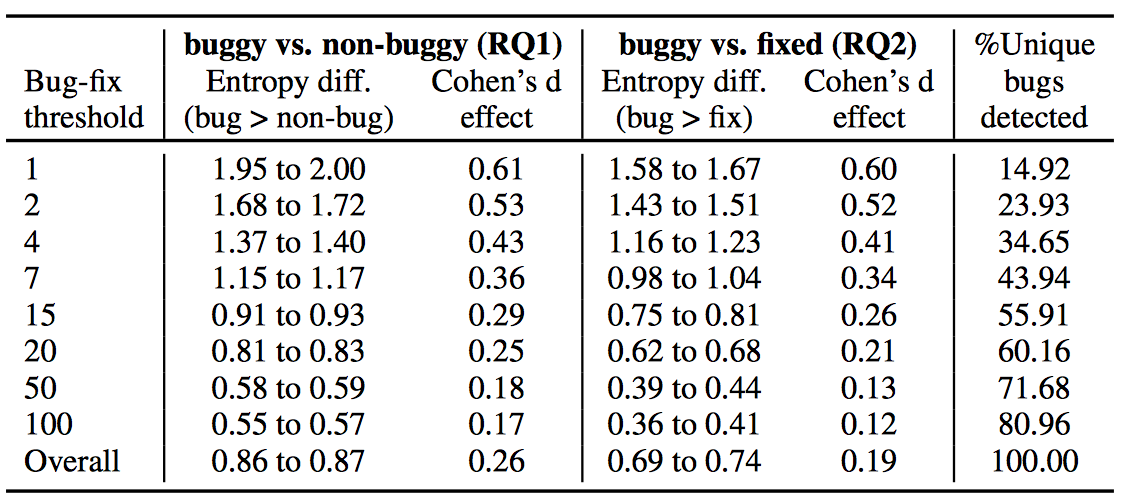
\includegraphics[width = \linewidth]{fig/entropydifference.png}
\caption{Bug和无Bug和修复后的熵的差异}
\label{fig:entropy_difference}
\end{figure*}
有Bug的行比没有Bug的行熵高,也比修复后的行的熵高。随着bug fix的阈值的增加,熵之间的差减小。

\textbf{研究问题1. 含有Bug的代码行会比没有Bug的代码行更加不自然吗?}

Bugs中的effect size比较小是因为受到了缠绕的Bug修复(tangled bug fixes),即在一次Bug修复提交中的行可能并不直接和这个Bug相关联。这种影响对于大型的Bug修复提交尤其明显,相比之下,小型的Bug修复提交,比如修复一或两行代码,那么这次修复的代码就很可能和这个Bug相关。

\begin{figure*}[!h]
\begin{tabular}{cc}
\subfloat[bug修复阈值为7时熵的差异]{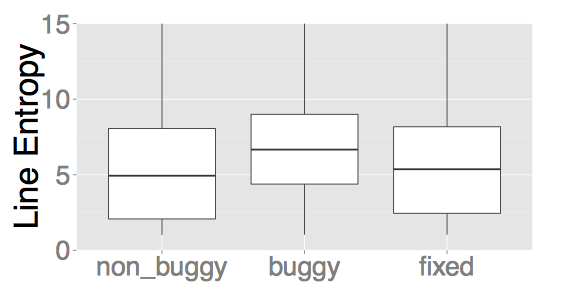
\includegraphics[width = 3in]{fig/threshold7.png}} &
\subfloat[不同bug duration的熵的差异]{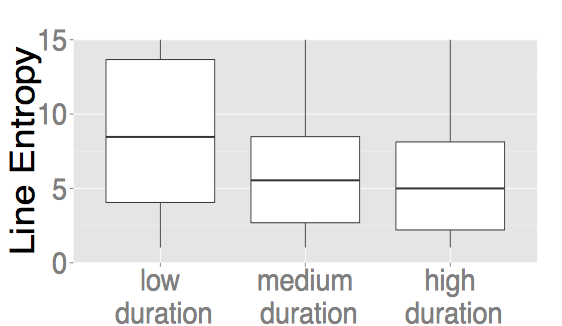
\includegraphics[width = 3in]{fig/bugduration.png}}
\caption{title}
\end{tabular}
\end{figure*}

为了了解缠绕改变对Bug代码自然性的影响,我们在不同的bug修复阈值计算bug代码和无bug代码的熵的差异。
bug修复阈值定义为在一次bug修复提交中从旧版本的一个文件中删除的行数。如图\ref*{fig:entropy_difference}所示。随着阈值的增大,熵的差别和effect size都在变小。如图(a)所示。这些结果表明:在缠绕bug修复提交中,与实际bug行间接相关的行可能具有较低的熵,从而降低bug行的总体熵。

另外,研究发现:在存储库中停留时间较长的bug,其熵值往往低于短期bug。bug存在时长为bug修复日期减去bug引入的日期。
基于bug duration,本文将所有的bug行分为三组:low, medium, and high。图(b)说明了他们之间熵的差异。

修复得越快的Bug比存在比较久的Bug更“不自然”。原因可能是:熵比较高的Bug比较容易定位诊断和修复。也有可能是:熵比较高的代码与用户更容易遇到的错误有更强的关联。
\textbf{一般来说,有bug的代码比没有bug的代码熵更高,更不自然。}

\textbf{研究问题2. bug修复后会变得更自然嘛?}
\begin{figure*}[!h]
\begin{tabular}{cc}
\subfloat[NBF成功检测到的bug修复提交,bug修复后熵变小]{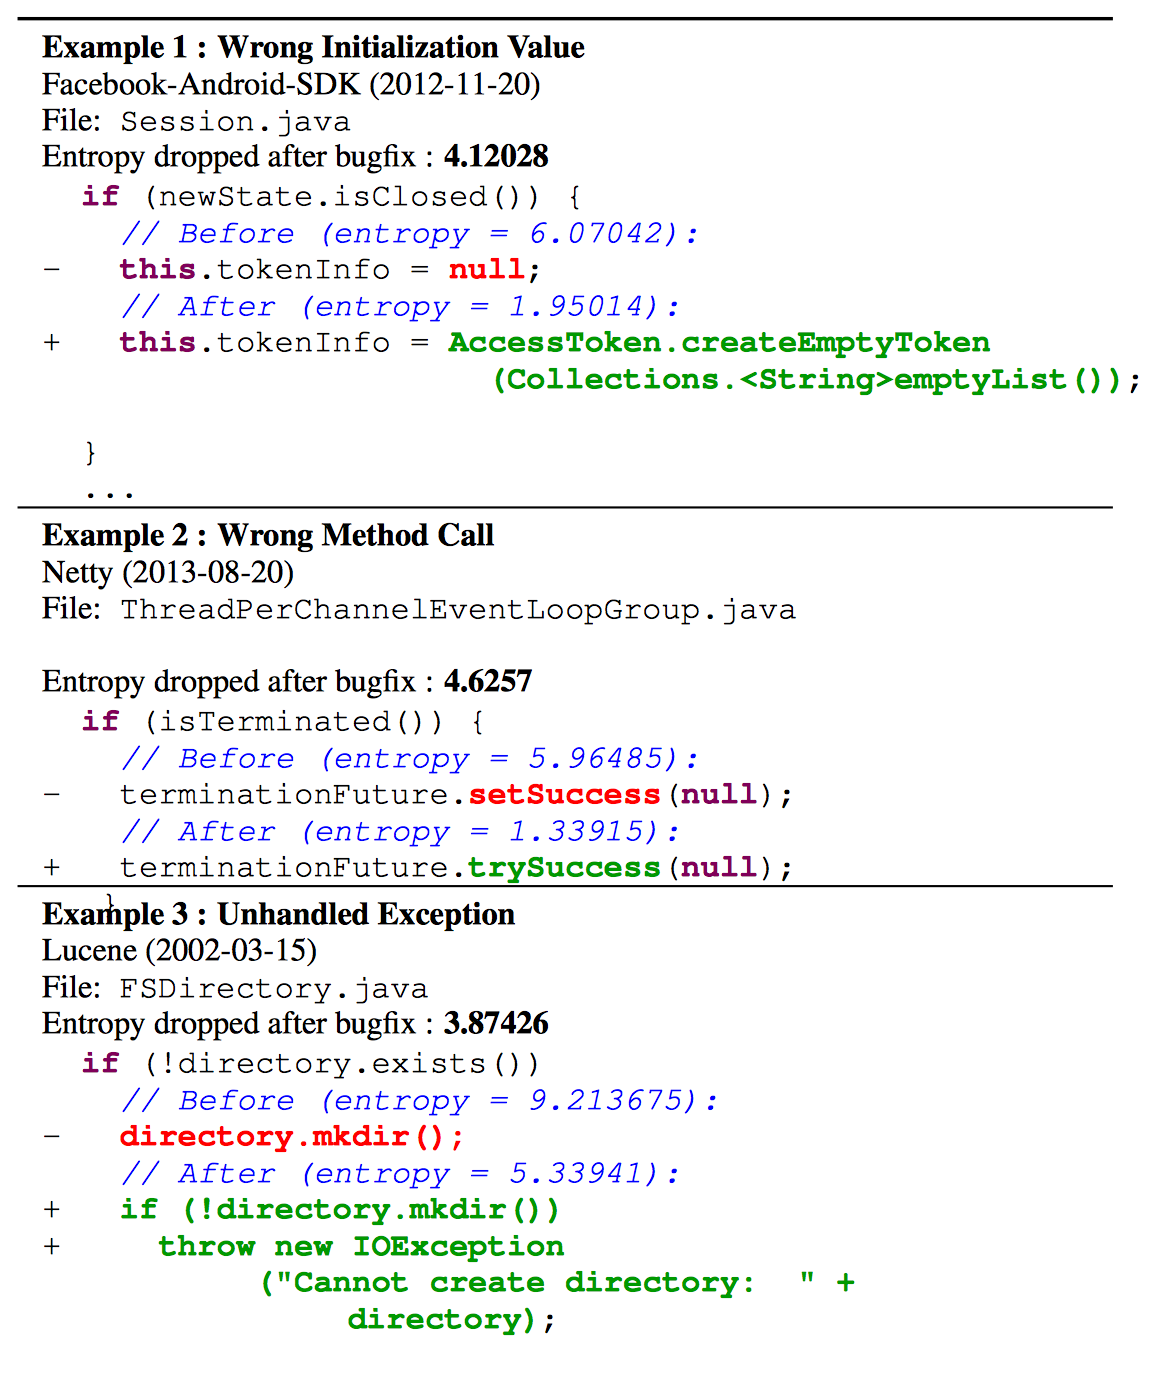
\includegraphics[width = 3in]{fig/table4.png}} &
\subfloat[NBF未能成功检测的例子]{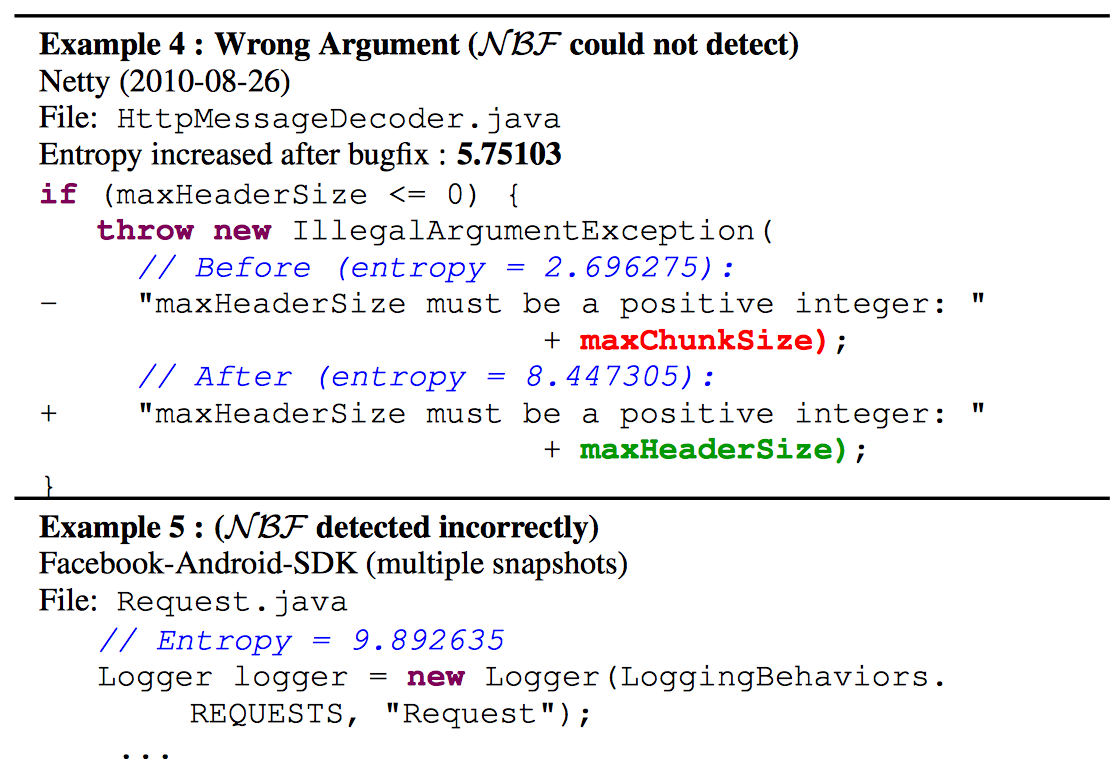
\includegraphics[width = 3in]{fig/table5.png}}
\caption{title}
\end{tabular}
\end{figure*}
\textbf{从统计学角度来说,在bug修复后含有bug行的熵变小了。}

\textbf{研究问题3. 自然性是否是一种检查编码工作的好的方式?}
\paragraph{文件级别}我们评估熵排序文件是否比传统的逻辑回归和基于随机森林的DP(缺陷预测)更好地指导我们识别错误文件。对于每个项目,我们在一个发行版上训练我们的模型,并在下一个发行版上进行评估:每个被测试的文件都分配了一个缺陷倾向性分数。我们对所有正在研究的项目重复这个过程。文件的熵是指文件中所有行的平均熵。

\paragraph{行级别}在说明了熵可以帮助检测容易出错的文件之后,我们现在关注的是一个更细的粒度:一行代码的熵可以用来指导对错误行的检查吗?具体来说,按熵排序的顺序会比随机排序更能指导检查工作吗?在我们所有的实验中,随机的基线选择线从未注释的源线(NCSL)中随机抽取,最多取NBF和SBF。

通过进一步的研究,我们发现一些程序结构本质上比其他的更熵。例如,方法声明通常更具有熵性,因为它们不太频繁。这个观察让我们考虑了错误预测中的句法线类型。按行类型划分熵值可以提高AUCEC的性能,并显著提高在所有情况下的性能,在这些情况下,$\$$gram的性能并不比随机的好。包括行类型的bug历史($\$$gram+wType),在除了Lucene和Atmosphere之外的所有代码中都优于random和$\$$gram,在bug-fix阈值为7时,AUCEC 5的总分比random高出92.53$\%$。由于$\$$gram+wType是迄今为止表现最好的“自然性”方法,我们将其称为NBF。

\textbf{熵可以用于在文件级和行级指导查找错误的工作。}

\section{总结}
代码的自然性表明,不自然的代码可能是错误的。本文使用语言模型度量熵,进一步作为一种度量自然性的一种方式。

本文研究发现,不自然的代码更有可能涉及错误修复,bug代码在修复后会变得更自然。然后本文将熵值应用到缺陷预测中,并且发现,当调整熵和缺陷发生的句法方差时,本文中使用的模型与常用的静态bug查找器PMD和FindBugs一样具有成本效益。将熵值(确定性)排序应用于这些静态bug查找器生成的警告,可以产生最具成本效益的方法。这些发现表明,熵值对缺陷预测方法可以有很大的帮助。研究结果还表明,某些基于自动搜索的bug修复方法可能在某种程度上受语言模型的影响。

\section{想法}
未来的编码工作是否能达到这样一个效果:程序员写完代码,IDE就会提示他,这里在将来运行时可能会出现Bug,请尽快修复,甚至可以直接提示修复建议。这个目前还是没有实现的,一般IDE提示的警告错误等都是基于语法分析,但是一些Bug的出现并不是因为语法错误,而是运行时错误,这个目前的IDE是没法做到的。我想能不能使用现在的机器学习方法再结合本文提出的代码自然性理论为每行代码计算熵值,并根据以前的历史数据来预测是否会出现Bug。

\newpage
\bibliographystyle{IEEEtran}
\bibliography{references}
\end{document}
